\documentclass[10pt]{article}

\usepackage[margin=1in]{geometry}
% https://tex.stackexchange.com/questions/27802/set-noindent-for-entire-file
\setlength\parindent{0pt}
% https://tex.stackexchange.com/questions/9550/why-does-underlined-text-not-get-wrapped-once-it-hits-the-end-of-a-line
\usepackage{soul}
\usepackage{indentfirst}
\usepackage{amsmath,amsthm,amssymb,scrextend}
\DeclareMathOperator*{\argmax}{arg\,max}
\DeclareMathOperator*{\argmin}{arg\,min}
% \usepackage{fancyhdr}
% \setlength{\headheight}{14.49998pt}
% \pagestyle{fancy}
\usepackage{graphicx}

\newcommand{\cont}{\subseteq}
\usepackage{tikz}
\usepackage{pgfplots}
\pgfplotsset{width=10cm,compat=1.9}

\usepackage{amsmath}
\usepackage[mathscr]{euscript}
\let\euscr\mathscr \let\mathscr\relax
\usepackage[scr]{rsfso}
\usepackage{amsthm}
\usepackage{amssymb}
\usepackage{multicol}

\usepackage{listings}
\usepackage{xcolor}
\usepackage{float}
\definecolor{codegreen}{rgb}{0,0.6,0}
\definecolor{codegray}{rgb}{0.5,0.5,0.5}
\definecolor{codepurple}{rgb}{0.58,0,0.82}
\definecolor{backcolour}{rgb}{0.95,0.95,0.92}

\lstdefinestyle{mystyle}{
    backgroundcolor=\color{backcolour},   
    commentstyle=\color{codegreen},
    keywordstyle=\color{magenta},
    numberstyle=\tiny\color{codegray},
    stringstyle=\color{codepurple},
    basicstyle=\ttfamily\footnotesize,
    breakatwhitespace=false,         
    breaklines=true,                 
    captionpos=b,                    
    keepspaces=true,                 
    numbers=left,                    
    numbersep=5pt,                  
    showspaces=false,                
    showstringspaces=false,
    showtabs=false,                  
    tabsize=2
}

\lstset{style=mystyle}

\DeclareMathOperator{\arcsec}{arcsec}
\DeclareMathOperator{\arccot}{arccot}
\DeclareMathOperator{\arccsc}{arccsc}
\newcommand{\ddx}{\frac{d}{dx}}
\newcommand{\dfdx}{\frac{df}{dx}}
\newcommand{\ddxp}[1]{\frac{d}{dx}\left( #1 \right)}
\newcommand{\dydx}{\frac{dy}{dx}}
\let\ds\displaystyle
\newcommand{\intx}[1]{\int #1 \, dx}
\newcommand{\intt}[1]{\int #1 \, dt}
\newcommand{\defint}[3]{\int_{#1}^{#2} #3 \, dx}
\newcommand{\imp}{\Rightarrow}
\newcommand{\un}{\cup}
\newcommand{\inter}{\cap}
\newcommand{\ps}{\mathscr{P}}
\newcommand{\set}[1]{\left\{ #1 \right\}}
\newtheorem*{sol}{Solution}
\newtheorem*{claim}{Claim}
\newtheorem{problem}{Problem}
\def\mathbi#1{\textbf{\em #1}}
\begin{document}

% \lhead{Stats 303}
% \chead{Luyao Wang lw337}
% \rhead{\today}

\begin{center}
  {\Large \bf COMPSCI 308: Design and Analysis of Algorithms Homework 5}
  \vspace{2mm}

  {\bf Luyao Wang}

  {\today}
\end{center}

\section*{1. Linear Programming (LP)}

\subsection*{(a) Solution Methods}

\begin{figure}[H]
  \centering
  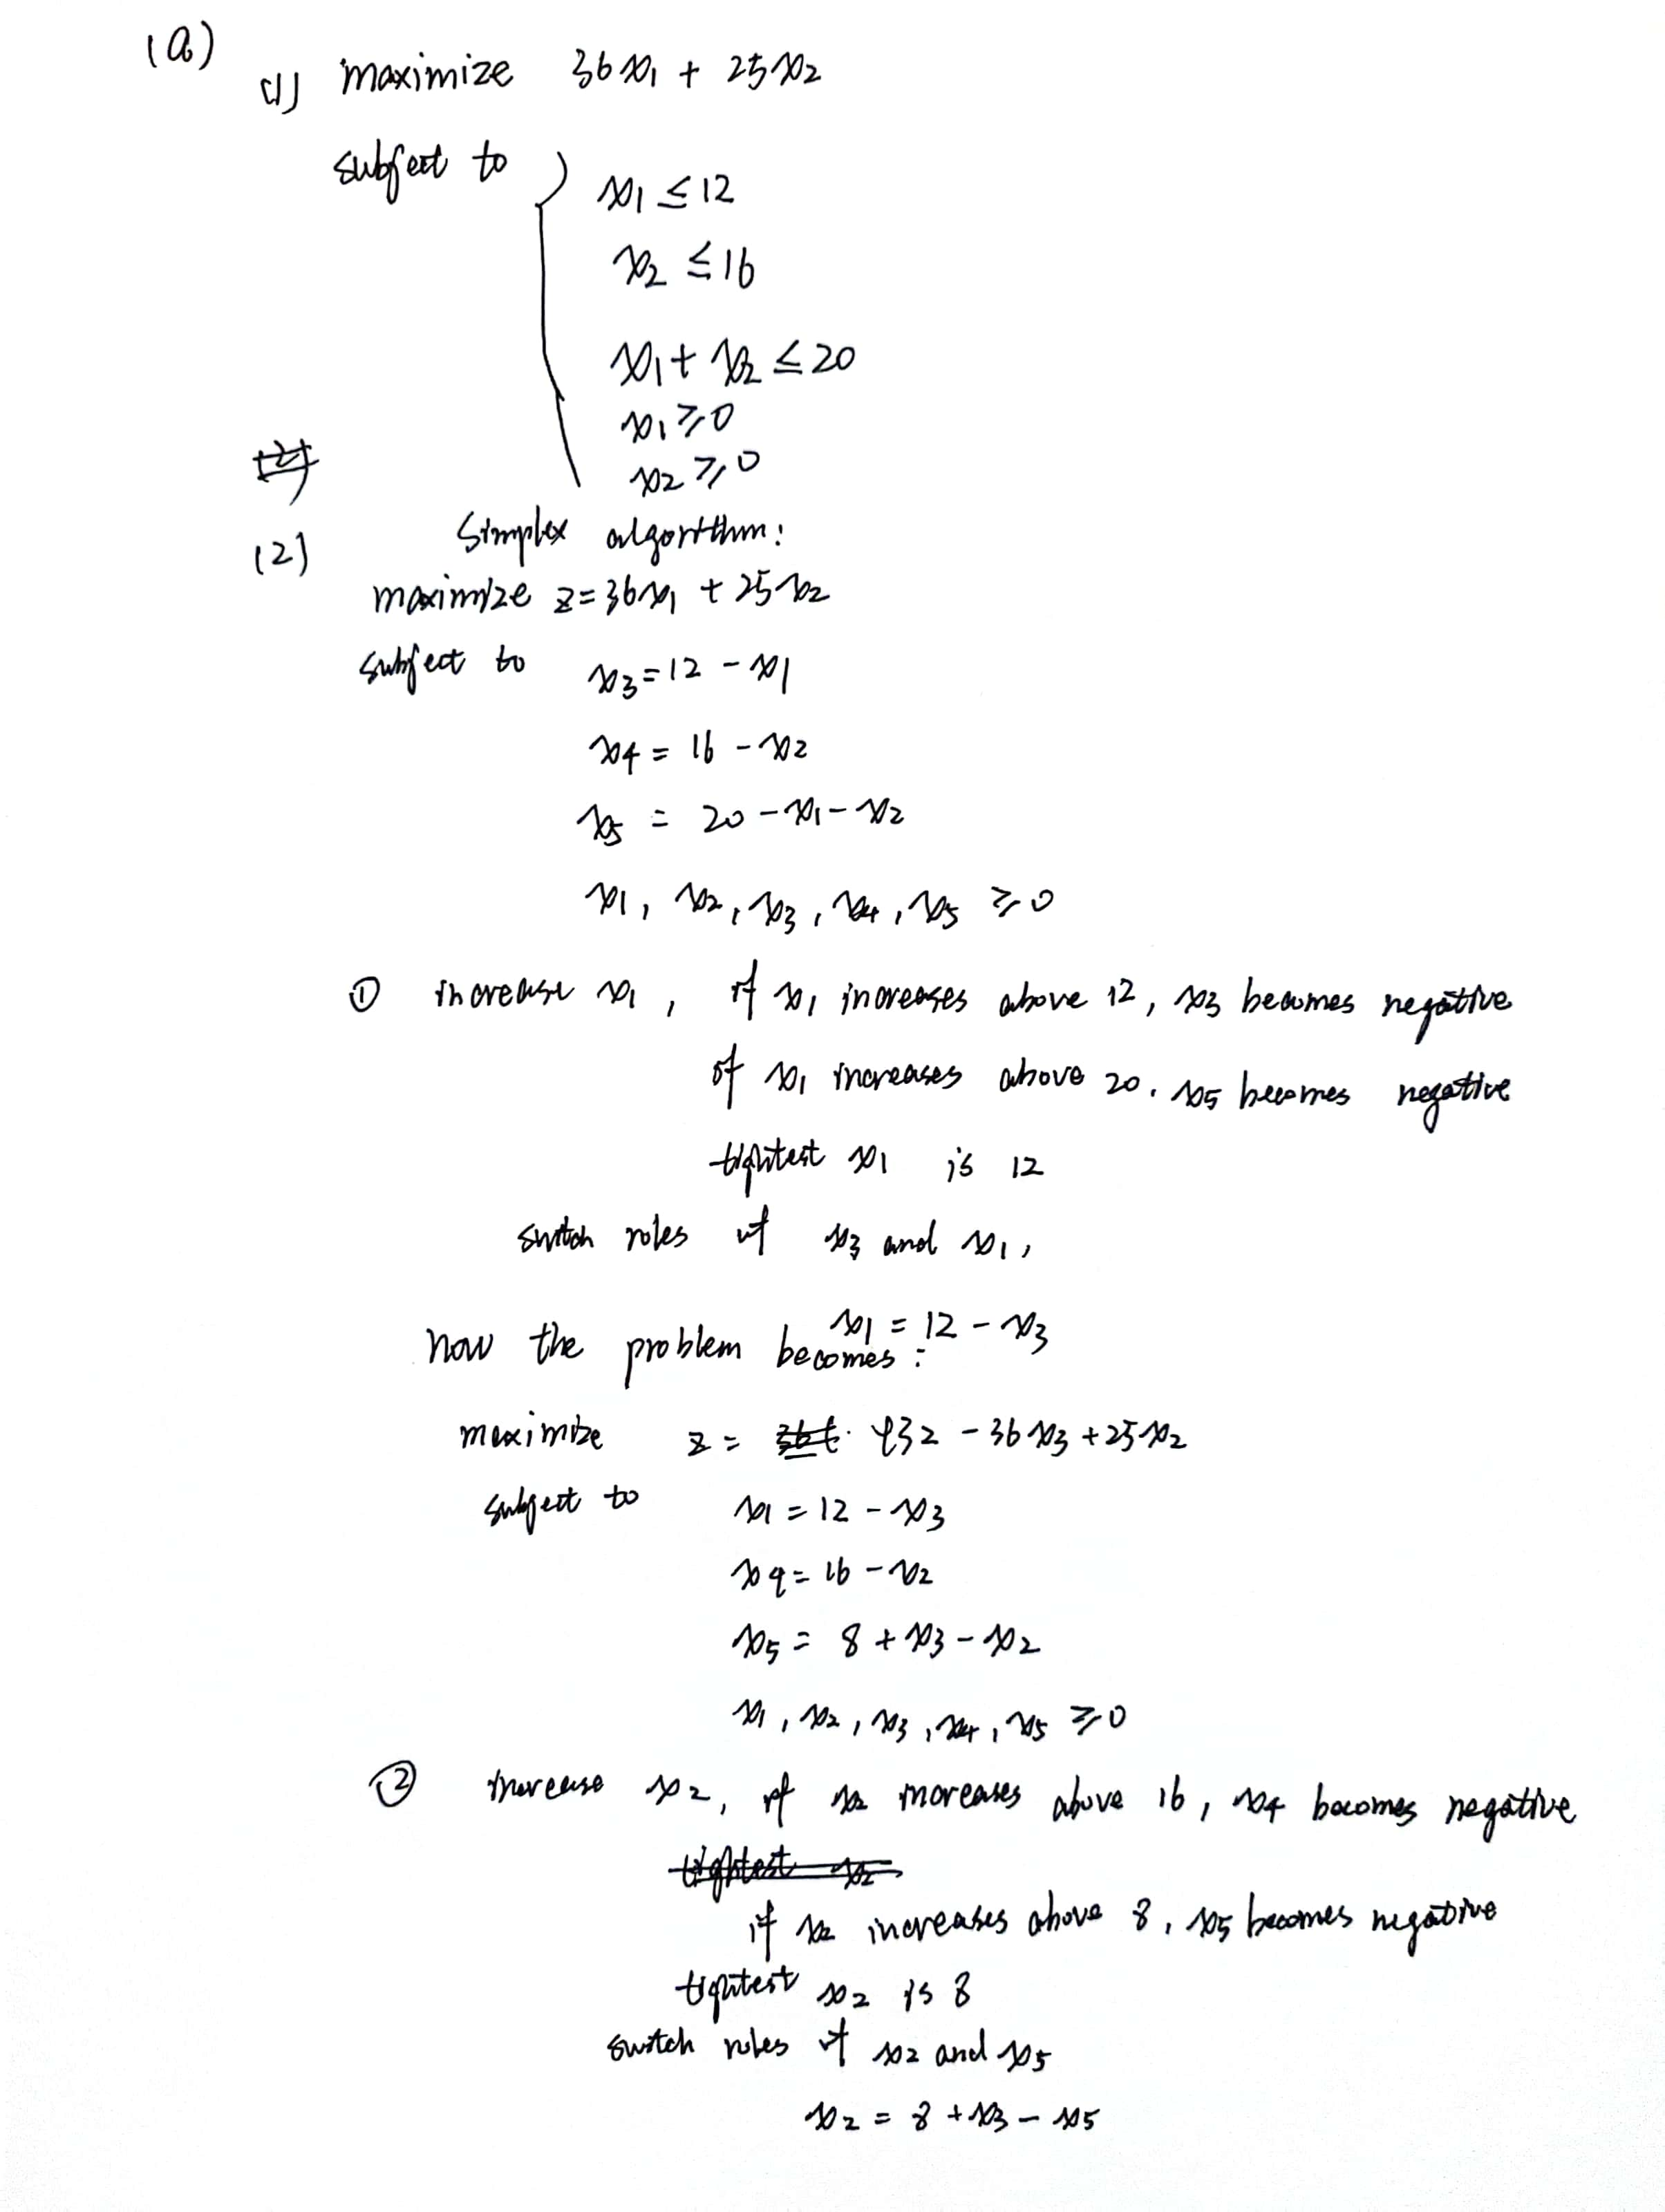
\includegraphics[width=\linewidth]{../assets/1.jpg}
\end{figure}

\begin{figure}[H]
  \centering
  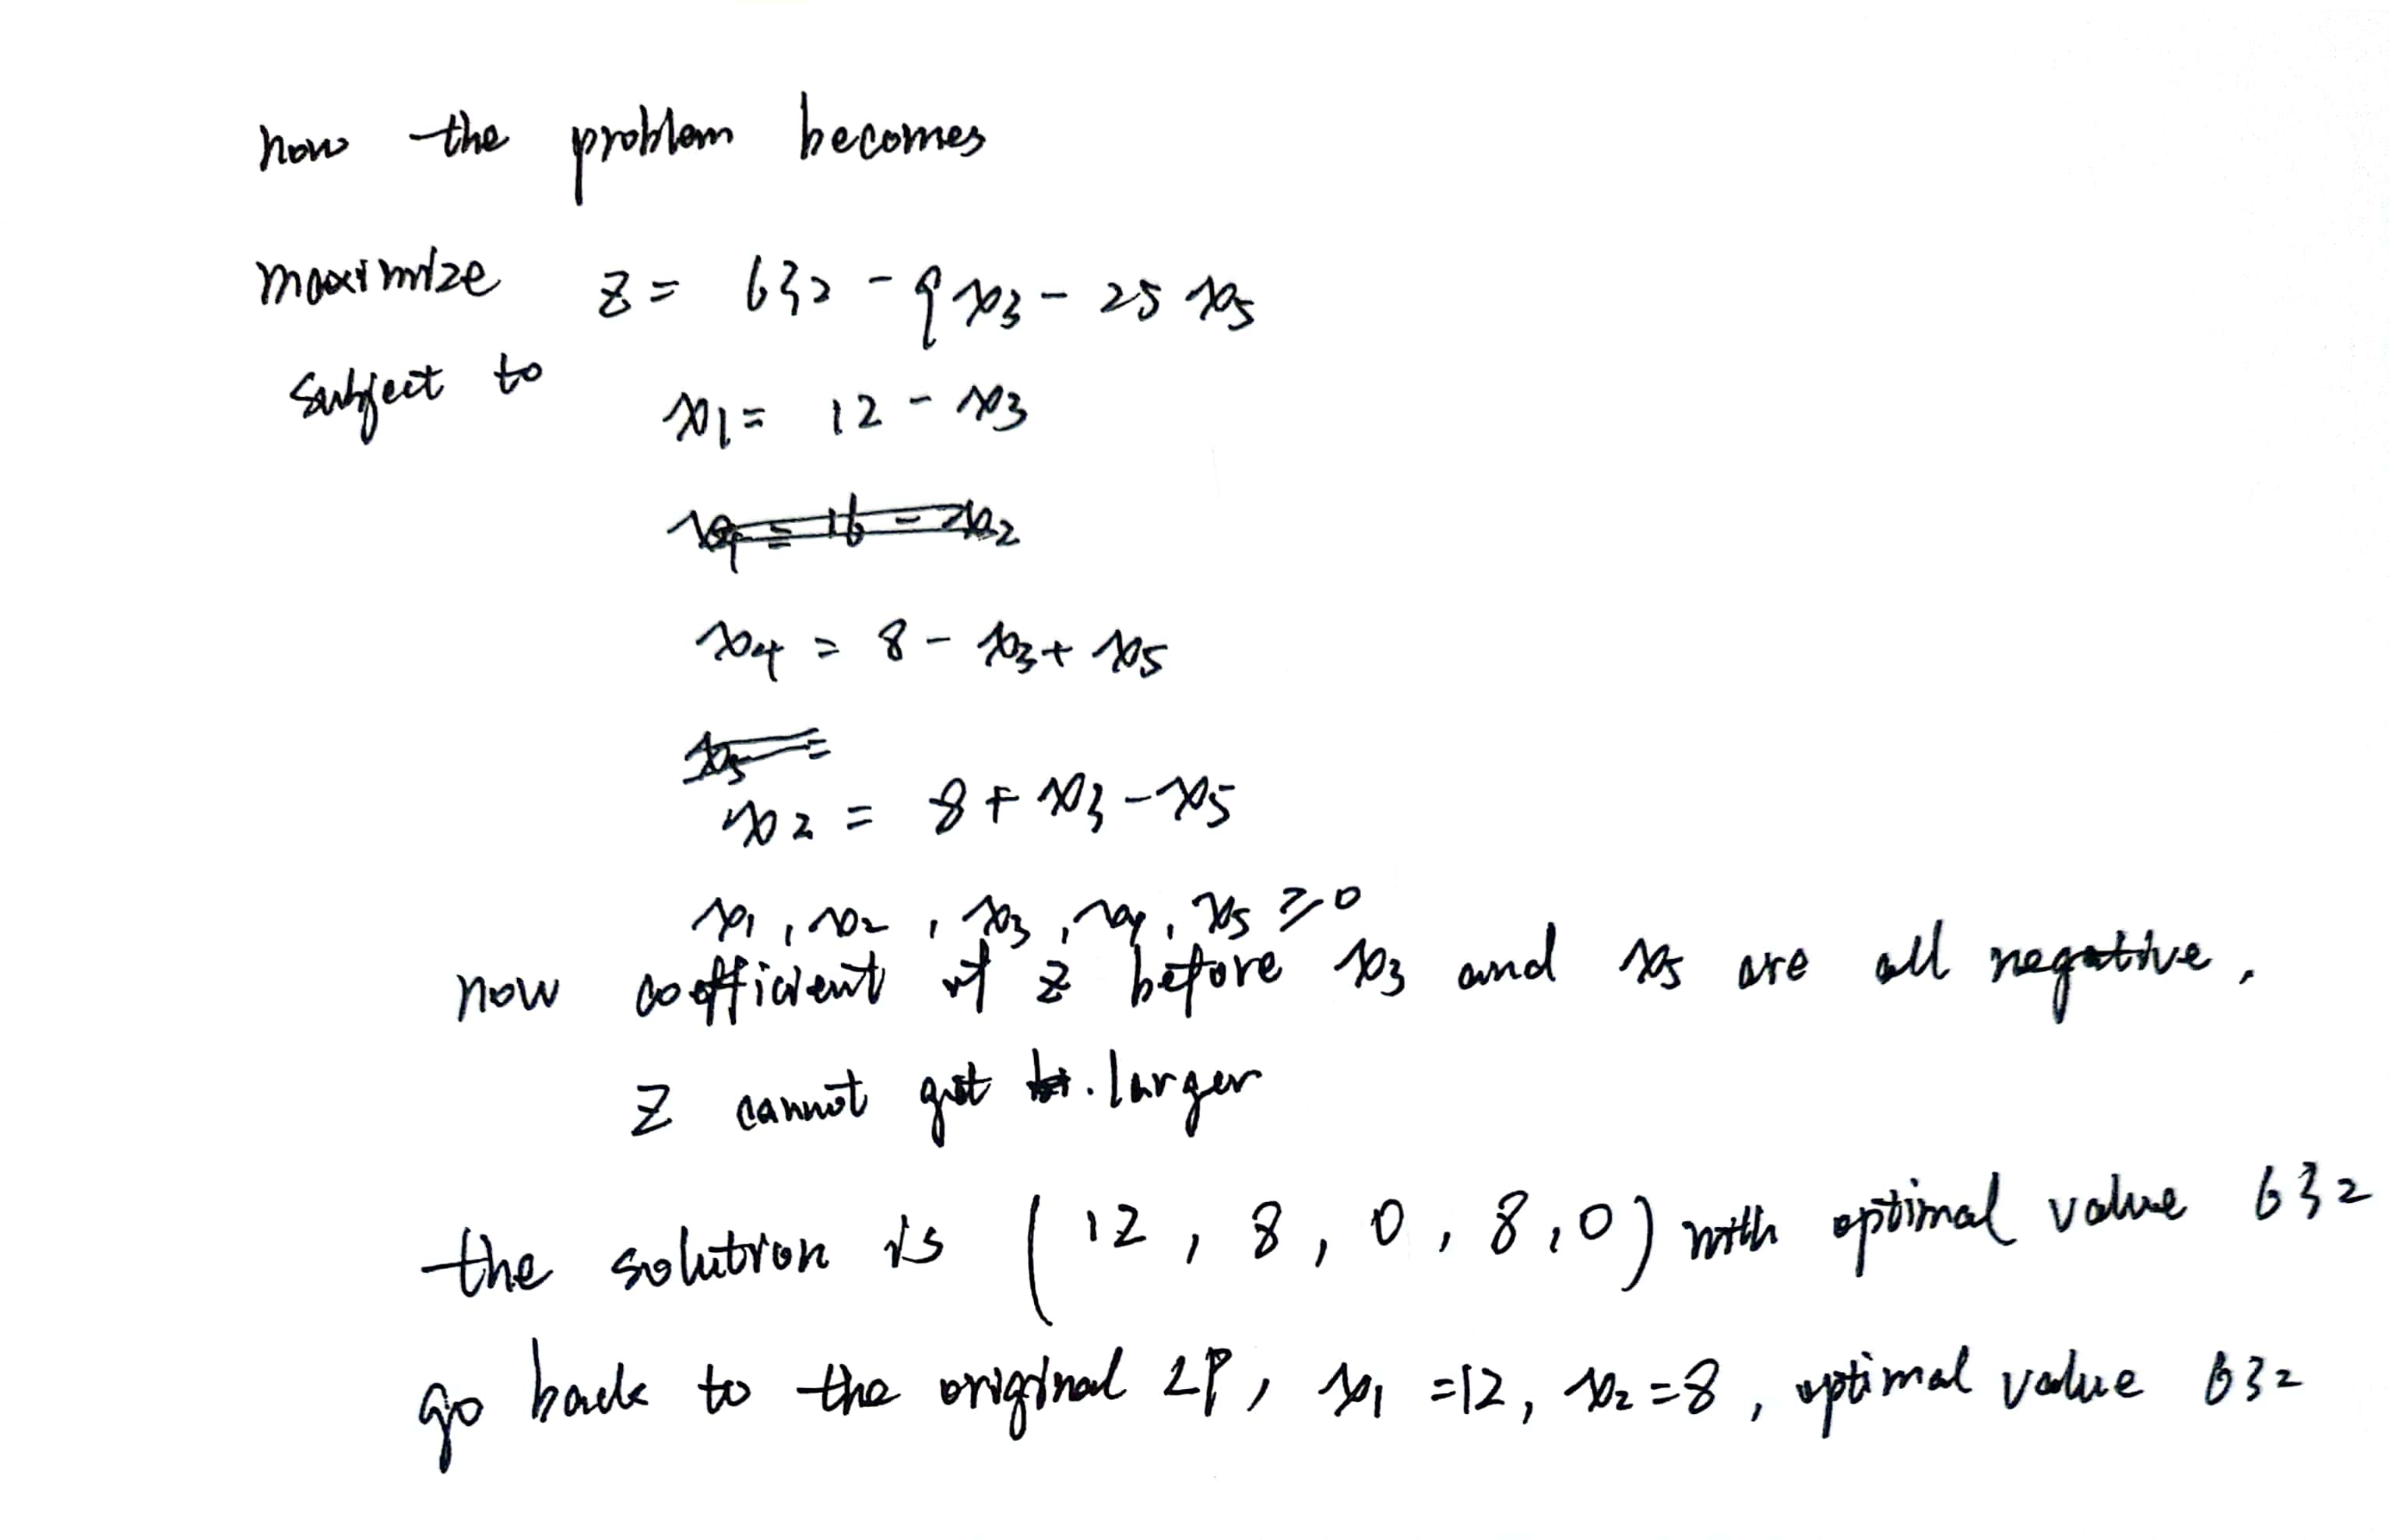
\includegraphics[width=\linewidth]{../assets/2.jpg}
\end{figure}

\begin{figure}[H]
  \centering
  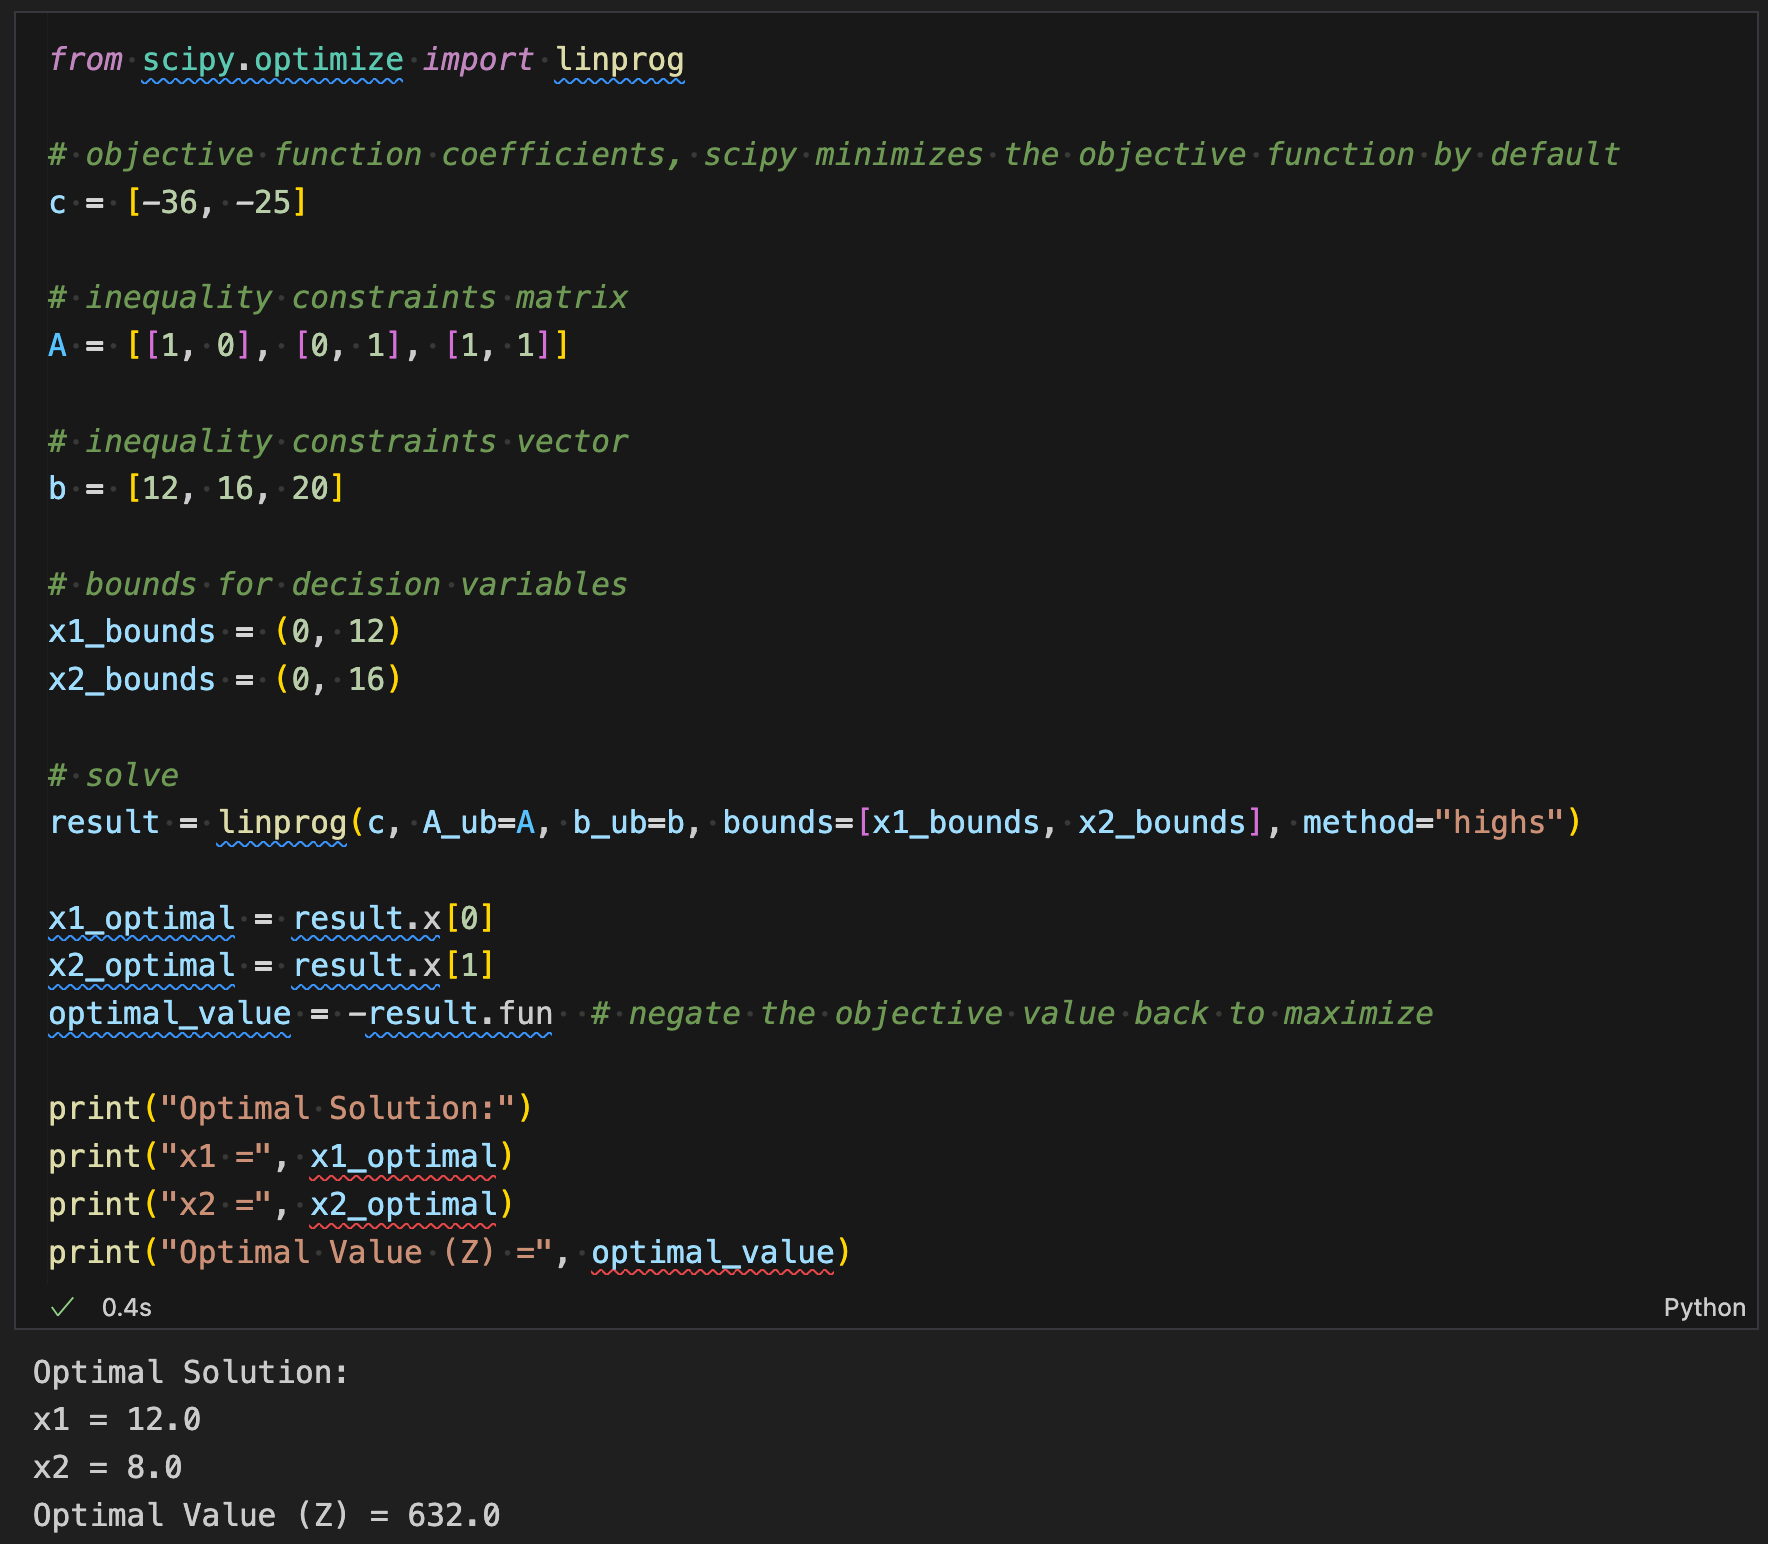
\includegraphics[width=\linewidth]{../assets/scipy_linprog.png}
\end{figure}

\begin{figure}[H]
  \centering
  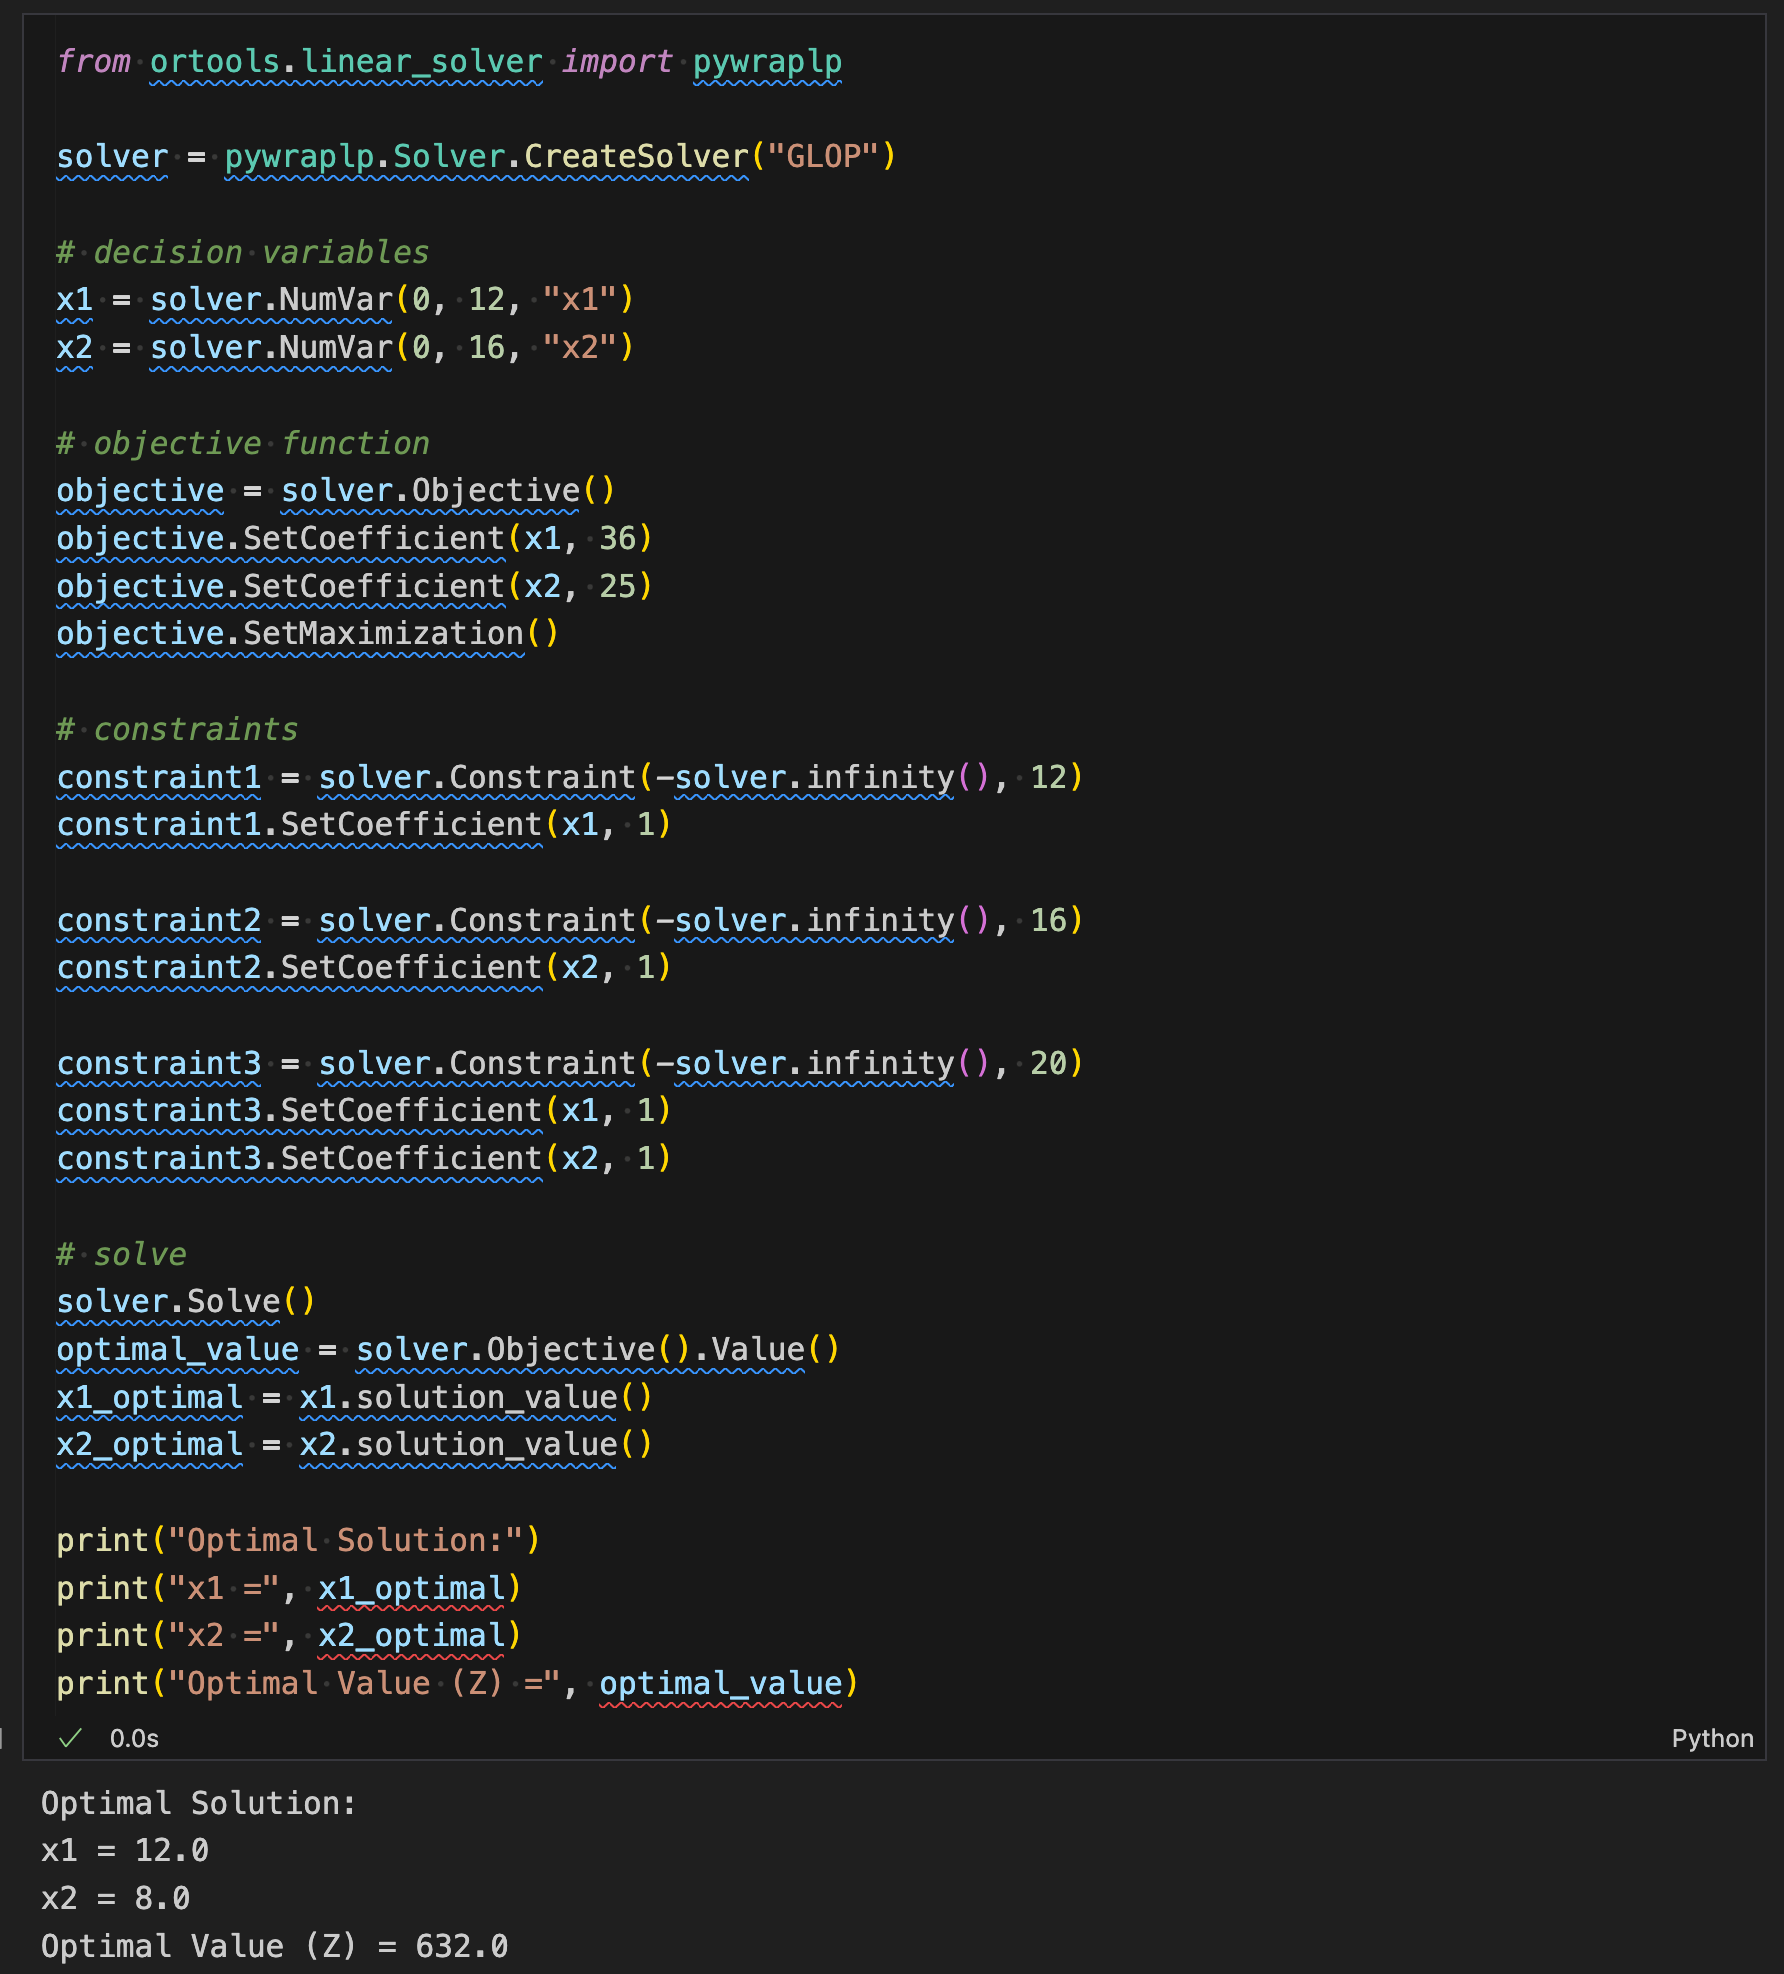
\includegraphics[width=\linewidth]{../assets/ortools.png}
\end{figure}

\subsection*{(b) Solution Space}

\begin{figure}[H]
  \centering
  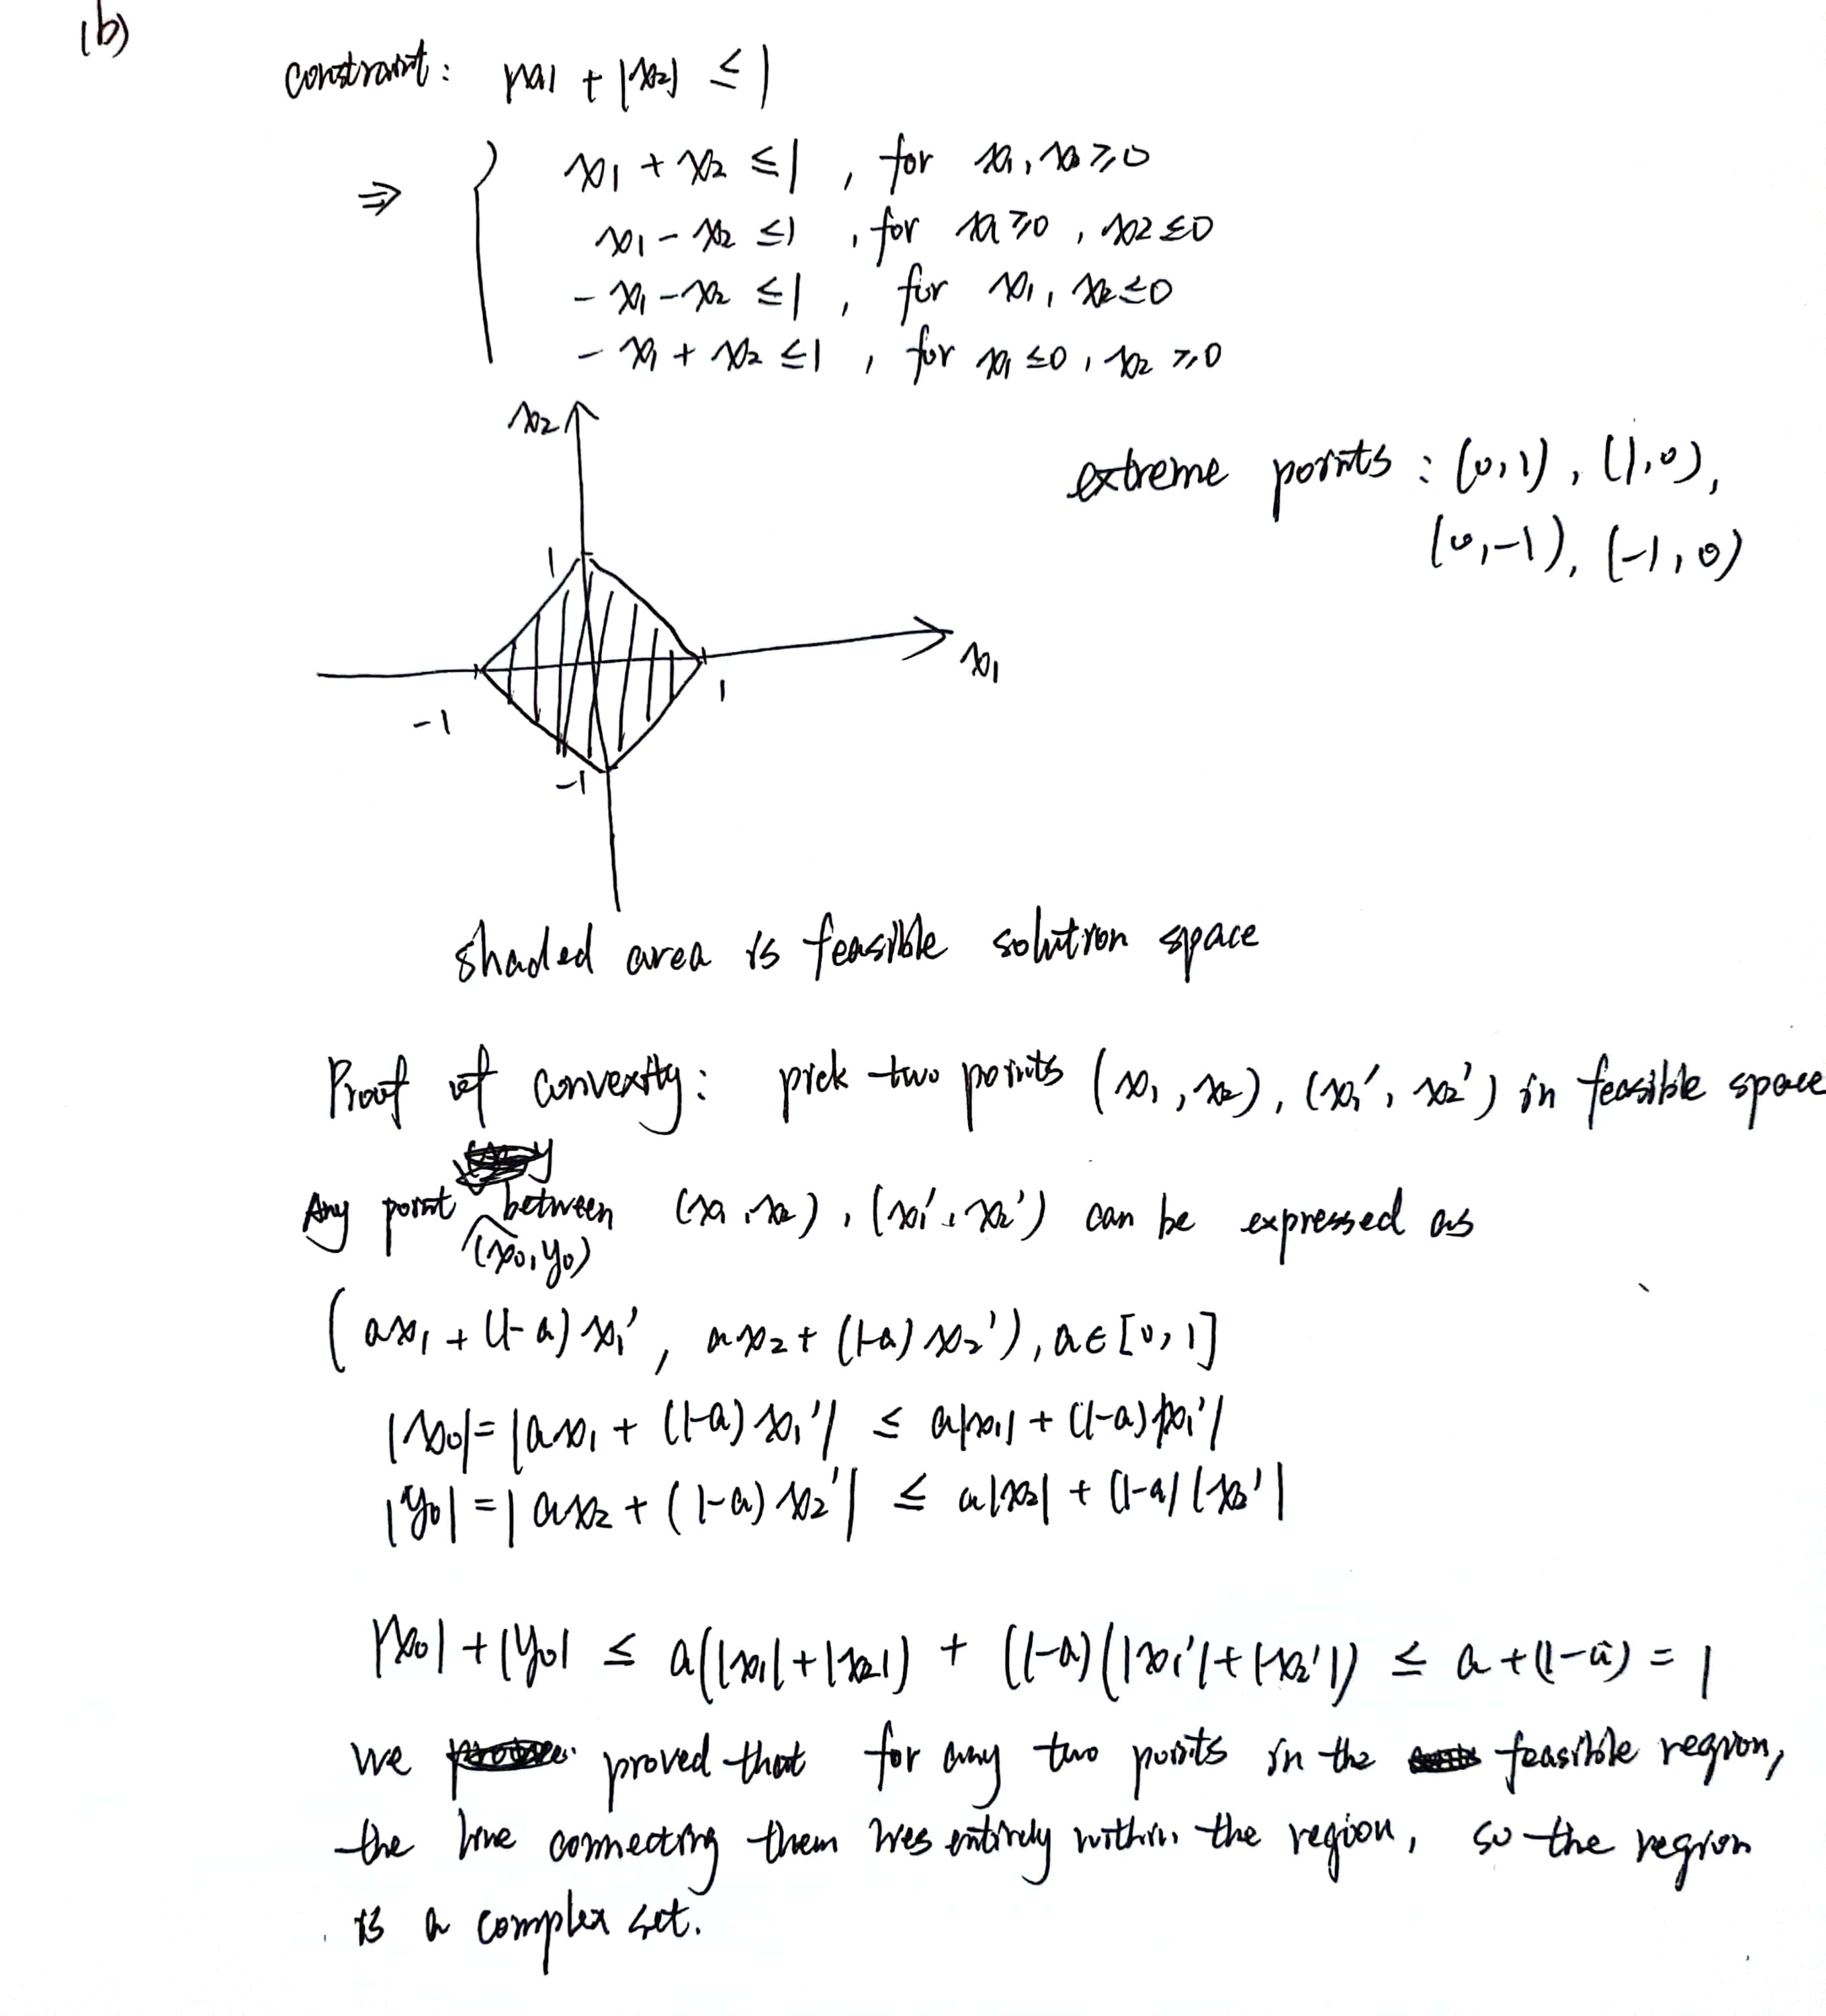
\includegraphics[width=\linewidth]{../assets/3.jpg}
\end{figure}

\subsection*{(c) Duality}

\begin{figure}[H]
  \centering
  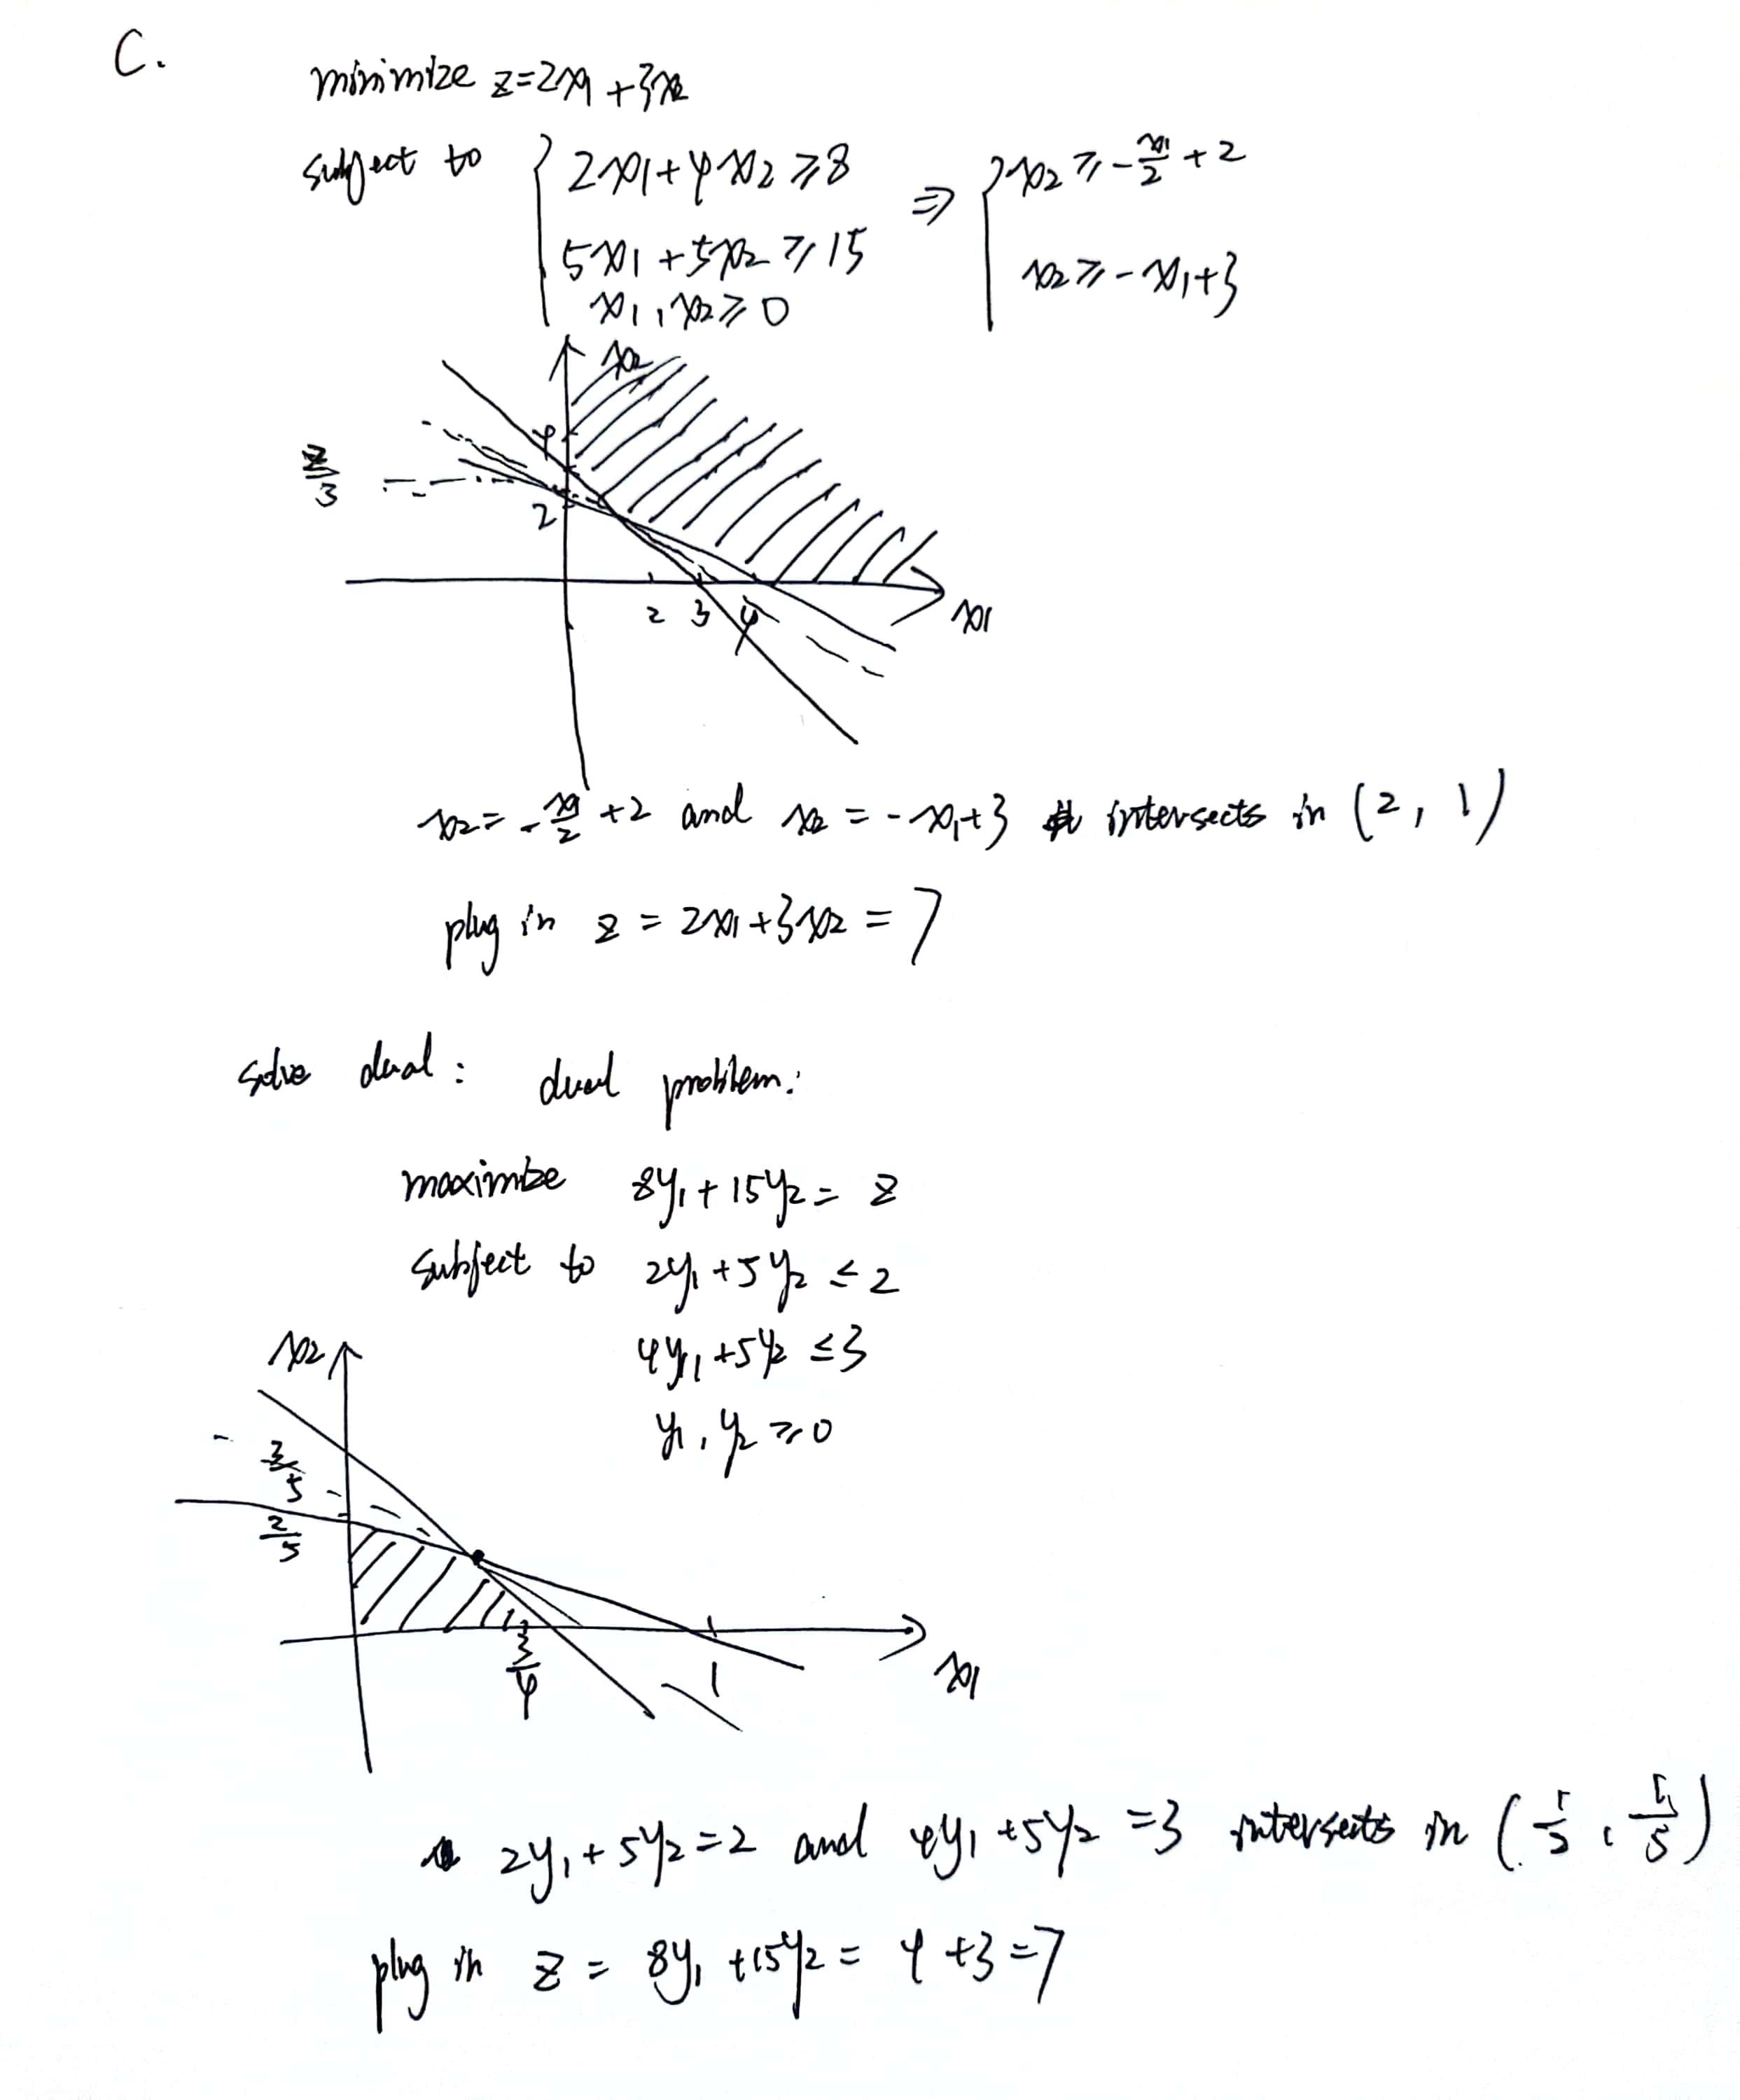
\includegraphics[width=\linewidth]{../assets/4.jpg}
\end{figure}

\end{document}